%!TEX root = ../username.tex
\chapter{Background}
\hspace*{-0.155cm}This chapter will provide the backgorund information necessary to understand what artificial reverberators are, why their use is important, and the different ways they are used by musicians today. It will begin with a broad definition of ``reverberation'' and discuss how sound persists in real-world spaces. After, it will discuss various methods of reverberating sound. Lastly, it will discuss how reverb is used today.

\section{What is Reverb?}
Imagine yourself speaking in a large concert hall. The audience does not only hear your voice; they hear the combination of both your voice and the reflections of your voice as they bounce off the walls and stage you are speaking on. In the right context, they serve both an artistic and practical purpose by enhancing the qualities of the sound being made on stage. In a broad sense, reverb can be defined as ``an ambient space in the perception of the listener'' \cite{dattorro1997effect}. This can take many different forms. Sound waves bouncing off the walls of a room, sound waves traveling through springs, sound waves traveling through a computer program - these are a few such ways in which a perceived ambient space can be created. It provides a texture that is considered ``wet'' and washes out the sound of an otherwise clear tone. In small amounts, it can be tasteful and enhance the timbre of an instrument. In large amounts, it can overpower the initial tone and can disrupt other elements of the music, such as rhythm \cite{blesser2007spaces}.

Consider an instrument with a short impulse response:

\begin{figure}[h] % [h] used to prevent {figure} from doing weird positioning
	\begin{center}
		\fbox{
		\begin{tikzpicture}
			\begin{axis} [
				axis x line = middle, % The x axis should go through the origin
				no markers,
				xlabel = \(t\),
				ylabel = {\(f(t)\)},
				height = 5cm,
				width = 12cm,
				xmin=0,
				xtick distance=0.2,
				]
				\addplot [
					red,
					thick
				] table [x=step,y=wav,col sep=comma] {test.csv};
			\end{axis}
		\end{tikzpicture}
		}
		\caption{A waveform of a snare drum.}
	\end{center}
\end{figure}

By adding reverb, this same instrument can sound as if it were performed in a large room:

\begin{figure}[h] % [h] used to prevent {figure} from doing weird positioning
	\begin{center}
		\fbox{
		\begin{tikzpicture}
			\begin{axis} [
				axis x line = middle, % The x axis should go through the origin
				no markers,
				xlabel = \(t\),
				ylabel = {\(f(t)\)},
				height = 5cm,
				width = 12cm,
				xtick distance=1,
				]
				\addplot [
					red,
					thick
				] table [x=step,y=wav,col sep=comma] {test2.csv};
			\end{axis}
		\end{tikzpicture}
		}
		\caption{A waveform of a snare drum with reverberation.}
	\end{center}
\end{figure} %fix to compress waveform to -1 and 1

Prior to the early 1960s, \textit{artificial reverberators} were physical devices - that is, something that took input from an electromechanical transducer and manipulated the sound using a variety of physical methods. Some such devices used metal plates, springs, and oil canisters - each providing their own unique sound and characteristics \cite{FiftyYears}. In some cases, these sounds were desirable and used for their specific timbral qualities. Some programs today aim to replicate the sound of these early devices. Many, however, prefer to mimic the sound that would be expected of a large hall, without any of the uniqueness of other methods. In 1961, M. R. Schroeder introduced a number of methods to digitally recreate reverb without additional color \cite{schroeder1961natural}. These same algorithms are used in several programs today.

\section{Historical Developments}
Prior to purely electronic means, there existed several methods of persisting sound with a short impulse. One such method is simply using a physical room. \textit{Echo chambers} are rooms constructed lacking parallel surfaces to effectively reverberate a sound \cite{FiftyYears}. They contain a speaker and a microphone to record the input signal once it has been reverberated, which is then mixed back with the original signal. Their primary benefit is derived from the method itself - using a real room will produce a sound that is indistinguishable to an otherwise reverberant hall. While echo chambers continue to exist today, their use is limited to those who have the infrastructure to build and maintain such rooms. They are most commonly found in recording studios, or otherwise special music production spaces. For individual devices, there are other methods of reverberating sound that are more convenient and cost effective.

\textit{Spring Reverberators} are another method. Their primary benefit is that they were compact - a much more convenient solution than an echo chamber. They were invented by Laurens Hammond after he patented the invention in 1941 \cite{laurens1941electrical}. In said patent, he describes a device in which sound traveling through a wire is sent through springs reinforced to the device, creating a reverberant sound. This reverberated signal is then sent back to be mixed with the original. Their small footprint allowed for their inclusion in devices such as synthesizers, a diagram of which can be seen below in Figure 2.3.

\begin{figure}[h] % [h] used to prevent {figure} from doing weird positioning
	\begin{center}
		\fbox{
		\includegraphics[width=16cm]{figures/elect.png}
		}
		\caption{A model of a Spring Reverberator \cite{devoe1977electronmusic}.}
	\end{center}
\end{figure}

Electromechanical devices such as these are not perfect, however. Their sound may provide an approximation of what might be heard in an echo chamber, but is not a perfect replication of the original. \textit{Plate reverberators} fall under a similar vein - sound travels through the plate and is mixed back with the original ``dry'' signal.

\section{How is Reverb Used Today?}
Nowadays, nearly every song one hears on the radio utilizes some kind of music application which allows one to record, edit, and manipulate several audio sources and recordings. Such applications are known as \textit{Digital Audio Workstations} (DAWs). By allowing the producer to manipulate recordings in real time, they can quickly and efficiently create the music that one hears today. DAWs accomplish this by providing tools to record the notes or sounds of instruments through various means. For example, virtual instruments stored on the producer's PC can be performed by a MIDI keyboard conneced to the DAW. These virtual instruments are known as \textit{plugins}, a type of application that runs under a DAW.

Plugins are generally broken into two distinct categories: \textit{generator plugins} and \textit{effect plugins}. Their difference is self-explanatory; generator plugins sample or synthesize a sound within the application, while effect plugins manipulate a given input. For the purposes of this thesis, focus will be placed on the development of \textit{effect plugins}. The producer can apply several of these effect plugins to a source sound in series. Effect plugins can range from distortion to chorus to arpeggiators, but they all operate using the same principle - take a signal as input, perform some type of operation to it, and return the processed signal. Reverb is one type of effect plugin that is often used in DAWs; an example of one such DAW can be seen in Figure 2.4.

\begin{figure}[h] % [h] used to prevent {figure} from doing weird positioning
	\begin{center}
		\fbox{
		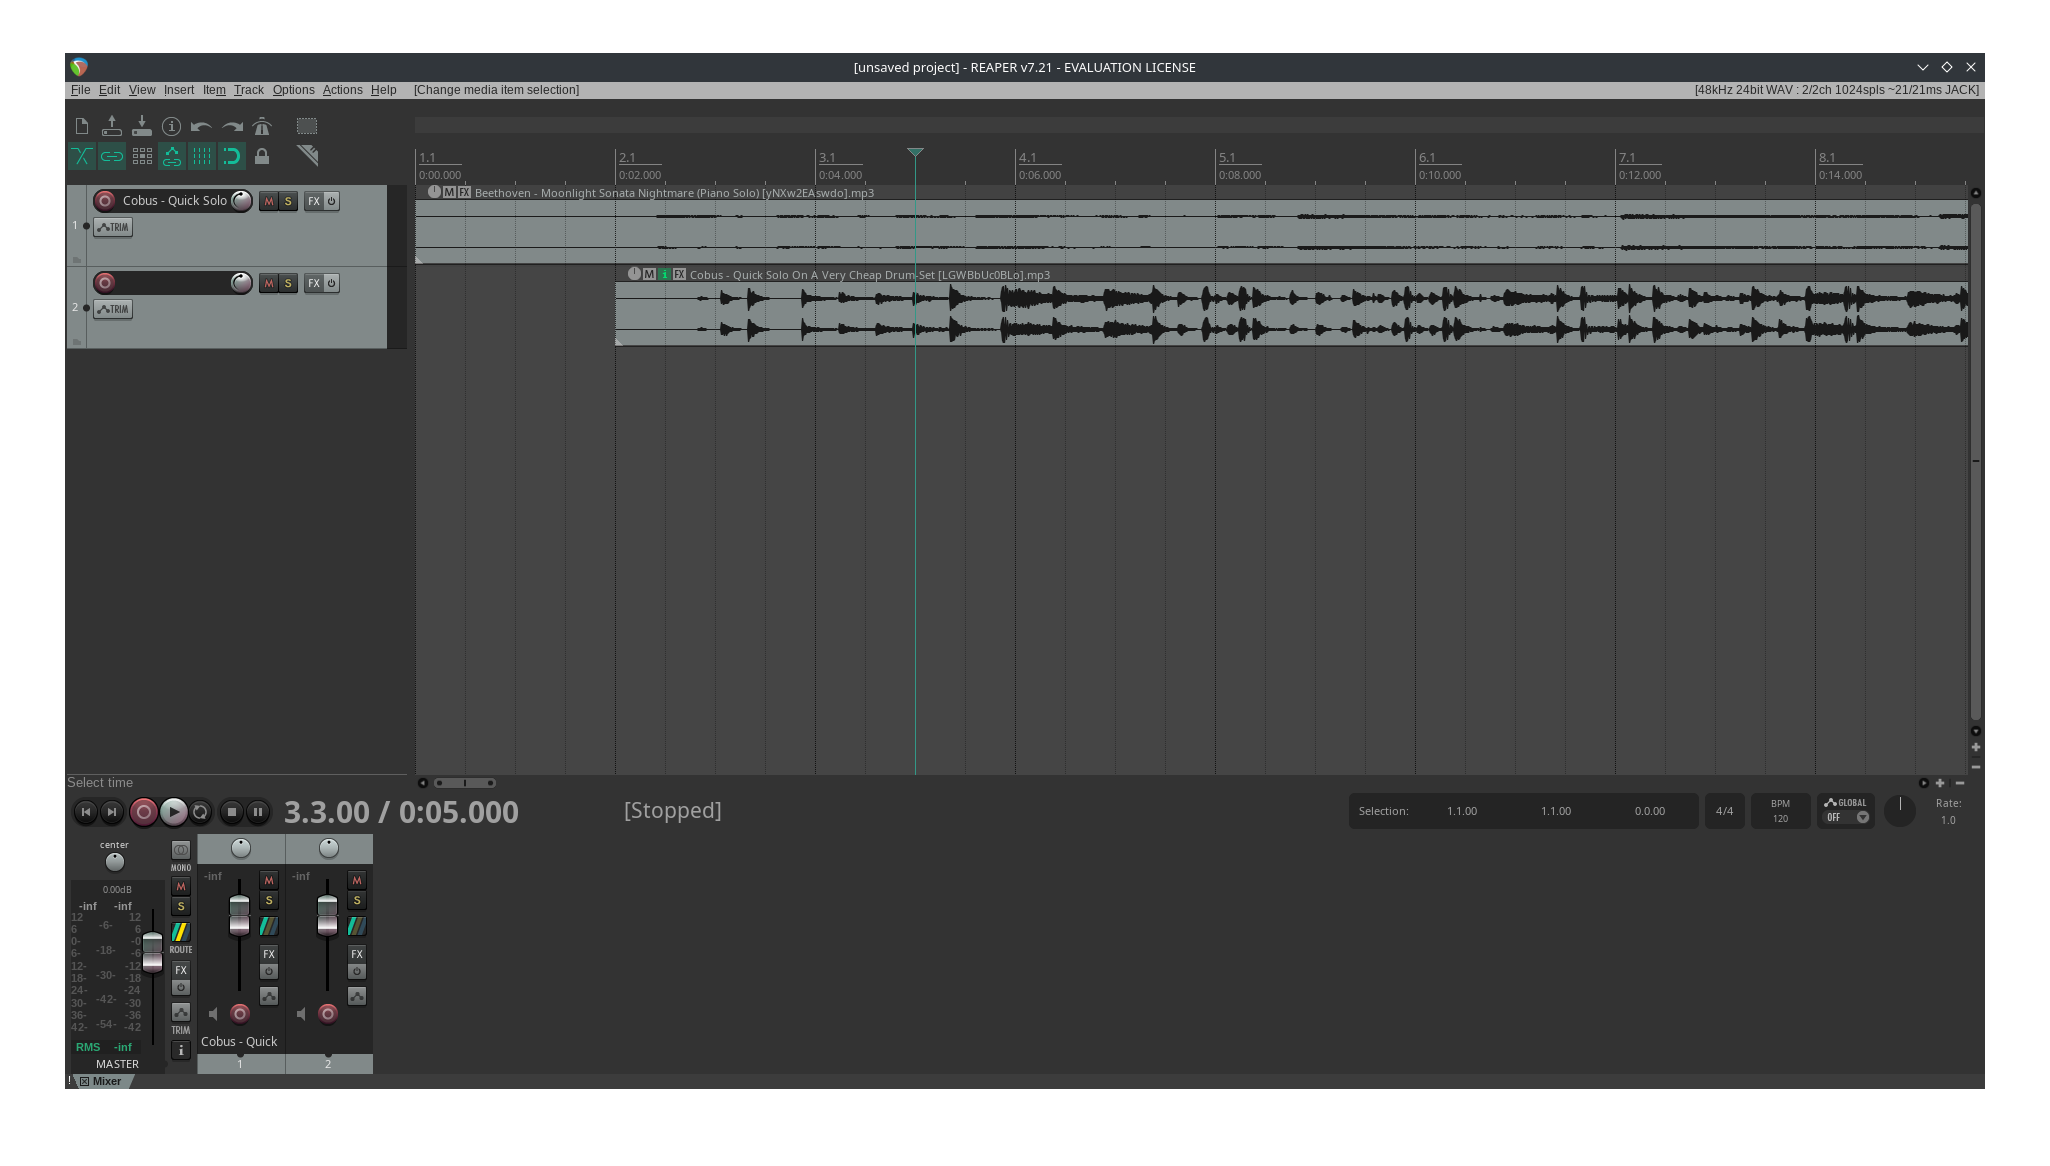
\includegraphics[width=16cm]{figures/DAW.png}
		}
		\caption{A screenshot of Reaper - a Digital Audio Workstation.}
	\end{center}
\end{figure}

While DAWs can differ in look and feel, they are generally broken into four separate areas:

\begin{itemize}
  \item The timeline: located in the middle, this contains each waveform and allows the producer to arrange how and when tracks are played.
  \item The track control panel: located on the left, this allows the producer to add and remove different tracks in a project.
  \item The mixer control panel: located on the bottom, this allows the producer to adjust the volume of individual tracks and add effects.
  \item The file explorer: not listed in the screenshot but commonly found, this allows the producer to browse samples and presets both included in the DAW and from their own filesystem.
\end{itemize}

These four sections are included in nearly every DAW available today. In practice, they allow producers to change when sounds occur and their volume by an exact amount. Through these tools, producers are able to create nearly any sound they can imagine; they can take parts of other songs and deconstruct them into something new; they can create an effect chain so complex that they turn a simple snare drum into something unrecognizable. The only limit is their creativity.
